\documentclass[11pt]{article}
\usepackage[margin=1in]{geometry}
\usepackage[T1]{fontenc}
\usepackage{lmodern,amsmath,amssymb,graphicx,booktabs,longtable,array}
\usepackage[hidelinks]{hyperref}
\usepackage{microtype}
\setlength{\emergencystretch}{3em}
\graphicspath{{figures/}}
\title{Independent reconstruction of the coastal adaptation model of Wong et al. (2025): continuing research report}
\author{Research-agent record prepared for Sophia Ludtke}
\date{12 October 2026}
\begin{document}
\maketitle
\begin{abstract}
Coastal cost distributions depend on both sea-level response and the joint
uncertainty assigned to climate, exposure, and adaptation. This project examines
whether the results of Wong et al.\ (2025) can be reconstructed from scholarly
documentation without consulting the authors' implementation or computational
outputs. We recover component equations, implement numerical kernels in Julia,
and compare manufactured cases with analytical limits and an independent SciPy
integration. Continued source recovery supplies coupled climate and Antarctic
dynamics, a closed carbon-cycle alternative, and independent observational inputs.
A temperature-only calibration passes convergence diagnostics but fails held-out
temperature and upper-ocean heat checks. These failures motivate a separate
temperature--heat calibration; they are retained as evidence of model limitations.
The calculations verify heat conservation, ice-response convergence,
flood-loss integration, and economic accounting. They also expose a finite-step
residual in the printed emissions recurrence and a lower-bound discrepancy in
an Antarctic temperature transform. These are findings about written equations,
not evidence of defects in the inaccessible original software. A complete
independent joint calibration and the target coastal input bundle were not
recovered. Consequently, none of the thirteen numerical target figures is
independently reproduced. An original workflow diagram, verified component
calculations, explicitly labeled alternative experiments, a complete figure register,
and recovery requirements document ongoing work. This report does not conclude
that all scientifically feasible reproduction work is exhausted.
\end{abstract}

\section{Objective and evidentiary boundary}

Wong et al.\ \cite{wong2025} estimate global coastal adaptation costs and losses
conditional on warming in 2100. Their model connects emissions, carbon cycling,
temperature and ocean heat, global and local sea level, and segment-level coastal
decisions. The scientific objective here is to reproduce the resulting
conditional distributions from the documented mechanisms. It is not sufficient
to draw curves resembling the published figures or to reproduce marginal
parameter ranges while discarding their dependence.

The independence restriction permits scientific papers, their supplementary
methods, and exogenous inputs from independent providers. Published figures and
printed summary statistics are comparison evidence only. No source code,
processed input bundle, posterior sample, simulation file, or plotting script
from the target authors was opened or used. An initial broad literature search
displayed incidental repository-index snippets, including a data-loading
excerpt. Those results were discarded, and subsequent searches focused on
scientific documents and provider records. This exposure is retained in the
research log rather than represented as complete isolation from search results.

The recovered sources include the target article and its ten-figure supplement,
the SNEASY climate description \cite{urban}, its carbon-cycle reference
\cite{ricciuto}, BRICK and MimiBRICK descriptions \cite{brick,joss}, the DAIS
paper \cite{shaffer}, and the CIAM mathematical supplement \cite{diaz}.
The December 2024 revision of the cited emissions preprint \cite{darnell} was
recovered through public scholarly file-version metadata. Its current DOI
landing page serves a later 2025 version. Since the target citation does not pin
a revision, this historical manuscript remains a version-qualified specification.
Stable acquisition URLs and hashes are recorded in \texttt{docs/SOURCES.csv}.

\section{Original experiment and recovered interfaces}

The target source ensemble contains 100,000 states of the world, with 5,000 used
for the coastal analysis. Global warming in 2100, relative to 1850--1900, defines
four bins: at most 1.5\,$^\circ$C, above 1.5 and at most 2.5\,$^\circ$C, above 2.5 and
at most 3.5\,$^\circ$C, and above 3.5\,$^\circ$C. Global sea level in 2100 uses a
1995--2014 reference. The baseline socioeconomic scenario is SSP4; SSP2 provides
a sensitivity case. Monetary outcomes are in 2010 US dollars with a 4\% annual
discount rate \cite{wong2025}.

The coastal model uses 12,148 DIVA segments and decadal calculations from 2010
through 2150. Planning intervals are 2010--2050, 2060--2100, and 2110--2150.
Protection and retreat standards are associated with return periods of 1, 10,100,
1,000, and 10,000 years, alongside no adaptation. The paper specifies nine
adaptation combinations. The complete 2022 scholarly supplement resolves the
menu: protection at 10--10,000 years and retreat at 1--10,000 years. The nominal
one-year level is annual maximum high tide, obtained for the GTSR experiment by
scaling the DINAS one-year level by the GTSR/DINAS 100-year ratio. It is not the
GEV quantile at probability zero.

The 2022 main methods specify first-period cost minimization, persistence of
the selected strategy and return level, and later height augmentation. Actual adaptation
already in place is not globally observed; the original calculation initializes
an optimal adaptation state. Reconstructing this spin-up requires the same
exposure and extreme-water inputs as the forward model. It cannot be inferred
from a global cost total.

Figure\ref{fig:workflow} identifies the implemented kernels and the missing
links. These kernels can be exercised independently. They do not constitute a
calibrated climate-to-cost simulation.

\begin{figure}[htbp]
\centering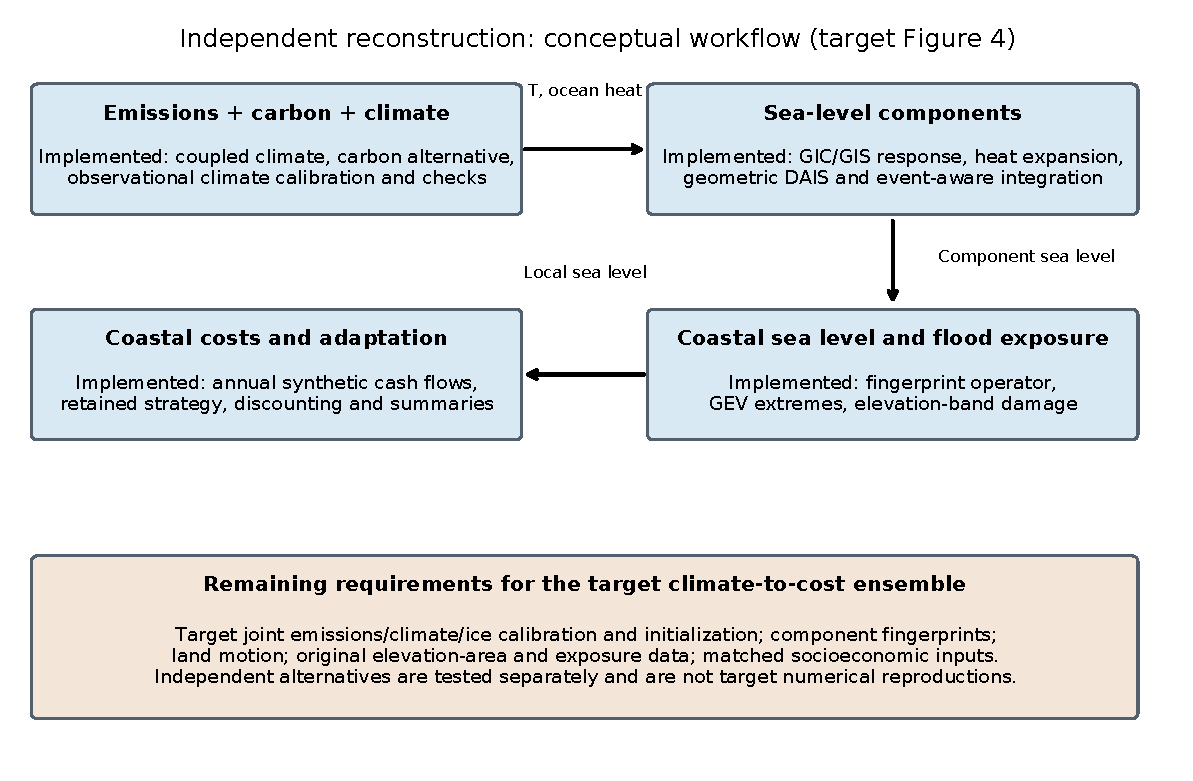
\includegraphics[width=\textwidth]{figure4_workflow.pdf}
\caption{Original conceptual schematic corresponding to target Figure 4.
Blue boxes identify implemented component calculations and their physical
interfaces. The lower box lists unresolved inputs and model closure. The arrows
describe required exchanges, not a claim that a complete coupled ensemble has
been executed. This diagram is not counted as a reproduced numerical result.}
\label{fig:workflow}
\end{figure}

\section{Independent mathematical reconstruction}
\subsection{Emissions and climate kernels}

For annual emissions $q_t$ in Gt\,CO$_2$\,yr$^{-1}$, the target's printed equation is
\begin{equation}
q_t=\begin{cases}
q_{t-1}+\gamma_g(\tau-t),& t\leq\tau,\\
q_{t-1}-2q_\tau\gamma_d e^{\gamma_d(t-\tau)}
             /[1+e^{\gamma_d(t-\tau)}]^2,&t>\tau.
\end{cases}
\label{eq:emissions}
\end{equation}
The implementation evaluates the second branch with negative exponential
arguments to avoid overflow while preserving the algebra. The growth coefficient
is interpreted in the annual recurrence's time convention; a dimensional
continuous-time growth coefficient would have different units. An integer peak
year is required explicitly. The emissions prior allows continuous peak years,
but the treatment of $q_\tau$ for a noninteger peak was not recovered.

The 2024 manuscript gives independent truncated-normal priors for growth,
peak year, and decline: means $(0.004, 2070, 0.07)$, standard deviations
$(0.0075, 25, 0.05)$, and bounds $[0.001,\infty)$, $[2030, 2200]$, and
$[0.001, 0.2]$, respectively \cite{darnell}. These are not the posterior
distributions used in the target ensemble. The subsequent inversion uses expert
cumulative-emissions information whose complete probability-density prescription
was not recovered. Sampling these priors would therefore not reproduce the
target emissions distribution.

Recoverable carbon kernels are net primary production
$N=N_0[1+\beta\ln(C/C_0)]$, with $N_0=60$\,Gt\,C\,yr$^{-1}$ and
$C_0=280$\,ppm, and heterotrophic respiration
$(a_1D+a_2S)Q_{10}^{\Delta T/10}$ \cite{ricciuto}. Here $D$ and $S$ are
detrital and soil carbon, and $a_1,a_2$ are turnover rates. The continuation
recovers terrestrial allocation and carbonate equilibrium, allowing the closed,
explicitly alternative calculation in Section\ref{sec:continuation}.
The implemented CO$_2$ forcing is $3.7\log_2(C/C_0)$\,W\,m$^{-2}$
\cite{urban}.

The ocean verification operator solves
$\partial_t T=\kappa\partial_{zz}T$ on a one-dimensional column with prescribed
surface temperature and zero bottom heat flux. Cell-centred finite volumes use
half-cell distance at the upper boundary. Backward Euler time integration
ensures that the column heat change equals the top flux evaluated at the new
time, to roundoff. Multiplication by volumetric heat capacity converts the
tested temperature integral to heat per unit area. This independently chosen
discretization is not asserted to match the original SNEASY solver.

\subsection{Sea-level components and spatial transformation}

The glacier contribution $S$ satisfies the documented reservoir relation
\begin{equation}
\frac{dS}{dt}=\beta(T-T_{\rm eq})(1-S/V_0)^n,
\qquad T_{\rm eq}=-0.15\,{}^\circ\mathrm{C}.
\end{equation}
Temperature is referenced to 1850--1870, $V_0$ is initial glacier volume expressed
as metres of sea-level equivalent, and $\beta$ has units m\,K$^{-1}$\,yr$^{-1}$
\cite{brick}. The numerical domain requires $S\leq V_0$ for fractional $n$.
An integration step that leaves this domain raises an error; no undocumented
volume clipping is introduced.

Greenland volume $V$, also in metres of sea-level equivalent, follows
\begin{equation}
V_{\rm eq}=cT+b,\qquad
\frac{dV}{dt}=(V_{\rm eq}-V)(\alpha T+\beta).
\end{equation}
The temperature reference is 1961--1990, and the volume loss relative to its
initial state yields sea-level rise. The rate $\alpha T+\beta$ must be
nonnegative. Constant temperature gives an exponential relaxation and therefore
an independent verification solution.

The target lineage uses a heat-driven thermal-expansion response,
$\Delta S_{\rm TE}=k_H\Delta H$, not the earlier temperature-relaxation emulator
\cite{vega,darnell}. The coefficient $k_H$ in m\,J$^{-1}$ remains an explicit
input. If the density expansion parameter $\alpha_\rho$ has units
kg\,m$^{-3}$\,K$^{-1}$, dimensional mass and heat accounting gives
$k_H=\alpha_\rho/(A C_p\rho^2)$. This is a dimensional derivation, not recovery
of a calibrated numerical coefficient. Supplying a conventional volumetric
coefficient in K$^{-1}$ in that expression would be a unit error.

The documented Antarctic ocean-temperature transformation is
\begin{equation}
T_o=T_f+\frac{x}{1+e^{-x/a}},\qquad
x=aT+b-T_f,\qquad T_f=-1.8\,{}^\circ\mathrm{C}.
\label{eq:anto}
\end{equation}
An additional threshold-triggered loss rate can be evaluated when its threshold
and rate are supplied. The continuation implements DAIS accumulation, marine
discharge and differentiated geometry from Shaffer\cite{shaffer}, with sign and
unit corrections derived explicitly. Present-day equilibrium and warming tests
verify these mechanisms. The target paleo calibration, initial state and full
coupling remain distinct recovery tasks. Land-water increments remain externally specified.

Local relative sea level is represented by
$L_i(t)=\sum_c F_{ic}S_c(t)+v_i(t-t_0)$, where $F$ contains component
fingerprints and positive $v_i$ increases relative sea level. This sign convention
includes subsidence as positive. The matrix operation is verified on known
area-weighted factors; actual fingerprint grids and coast matching are absent.
Reference-period routines require complete annual coverage and refuse silent
rebasing of an incomplete series.

\subsection{Coastal damage and costs}

The independently implemented flooding calculation uses a generalized extreme
value (GEV) distribution for annual extreme water level and piecewise uniform
area density within supplied elevation bands \cite{diaz}. For water height $w$
and exposed elevation $e$, property damage is proportional to
$\phi(w-e)=(w-e)/(h_0+w-e)$ with $h_0=1$\,m. The integral over an exposed
band $[a,b]$, where $b\leq w$, is
\begin{equation}
\int_a^b\phi(w-e)\,de=(b-a)-h_0\ln\!\left(\frac{h_0+w-a}{h_0+w-b}\right).
\end{equation}
Multiplication by area density and capital density yields event loss. Mortality
uses flooded population, a supplied mortality fraction and value of statistical
life. Both contributions are multiplied by $1-r$, where $r$ denotes economic
resilience. Integration of this loss against the GEV density produces expected
annual loss. The surge integration bound is explicit, and the truncated density
is not renormalized. Retreat changes the lowest retained elevation; protection
changes the overtopping threshold.

Relocation combines income-related moving cost, mobile-capital transfer cost,
and demolition of immobile capital. The documented benchmark mobile share is
one quarter; immobile capital is three quarters. Reactive relocation costs five
times the proactive counterpart in the target model. Separate kernels calculate
inundation with explicit depreciation, wetland loss with a critical rise rate,
and quadratic-height seawall construction. Annual maintenance is returned as
a separate cash flow. The numerical coefficient in the construction formula
must have units consistent with its quadratic height dependence; the quoted
historical reference cost is not silently substituted where its unit convention
is ambiguous.

For annual payments $C_y$, the explicit discount operator is
\begin{equation}
\mathrm{PV}_{y_0}=\sum_y\frac{C_y}{(1+r)^{y-y_0}}.
\end{equation}
A 2010 base year and 4\% rate are used in verification. This base-year convention
does not resolve the target caption's wording about discounting through/to 2150.
The optimizer chooses the least-cost member of a supplied finite candidate
menu. It does not construct the original adaptation trajectories, because their
physical and socioeconomic inputs are missing.

\section{Verification results}

All 80 original Julia assertions pass across seven groups: emissions/carbon/forcing;
ocean conservation and convergence; sea-level limits; spatial accounting and
references; extreme levels and damage integration; costs and optimization;
and ensemble/regional arithmetic (the sea-level group includes ODE accuracy).
These original tests are numerical verification tests. Additional mechanism tests
and observational checks are described in Section\ref{sec:continuation}.
The tests require no third-party Julia packages. Configuration values are
explicitly marked as manufactured in \texttt{config/validation.toml}.
Table\ref{tab:metrics} is generated directly from the diagnostic files and the
independent SciPy checks.

\begin{table}[htbp]\centering\small
\begin{tabular}{p{0.70\textwidth}r}\toprule
Verification quantity & Calculated value\\\midrule
Greenland finest absolute error (m SLE) & 5.398e-10 \\
Ocean finest maximum temperature error (K) & 6.759e-06 \\
Ocean maximum heat-balance residual (K m) & 1.021e-16 \\
Expected flood loss, SciPy reference (USD/year) & 442422.479342 \\
Expected flood loss, Julia relative difference & 1.271e-11 \\
Depth integral maximum difference (USD) & 9.313e-10 \\
Annual emissions residual at gamma=0.07 (\% of peak) & 1.750000 \\
Minimum sampled Antarctic ocean transform (degree C) & -2.078464 \\

\bottomrule\end{tabular}
\caption{Computed verification metrics. These quantities describe manufactured
test cases, not target global projections. The heat-balance residual is reported
before multiplication by volumetric heat capacity.}\label{tab:metrics}
\end{table}

\subsection{Printed emissions recurrence and its limit}

Figure\ref{fig:emissions} compares the literal recurrence with the continuous
logistic decline $q(t)/q_\tau=2/[1+e^{\gamma_dt}]$. The decrement in
Equation\ref{eq:emissions} is the right-endpoint sample of the continuous
decline rate. Summing endpoint samples does not exactly integrate that rate.
For small step $\Delta t$, the residual fraction is
$\gamma_d\Delta t/4$ to leading order. At an annual step and decline rate
0.07\,yr$^{-1}$, the calculated residual is approximately 1.75\% of peak
emissions. The tested rates 0.01 and 0.2\,yr$^{-1}$ give approximately 0.25\%
and 5\%, respectively. Refining the quadrature step reduces the residual.
These are normalized mathematical cases extending 2000 years after an arbitrary
peak, not calendar-year emissions projections.

The discrepancy separates two interpretations of the published specification:
literal annual accumulation and a continuous logistic trajectory that vanishes
asymptotically. No choice was imposed on a global simulation. The effect on
temperature and costs cannot be calculated without the missing coupled model.

\begin{figure}[htbp]\centering
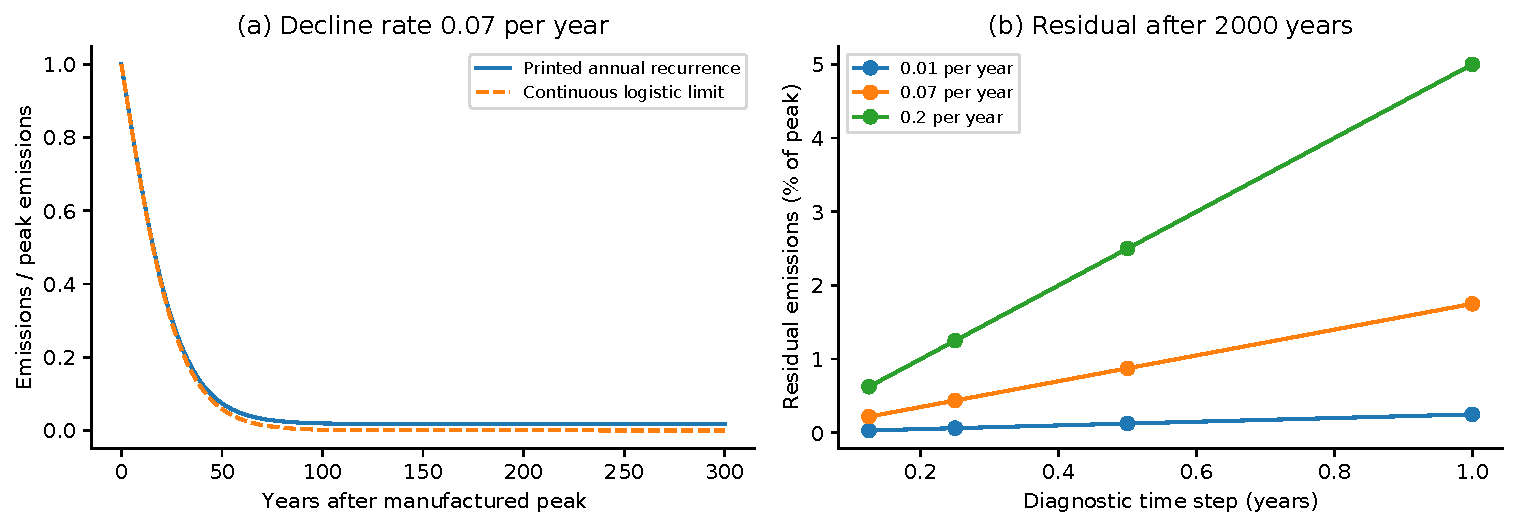
\includegraphics[width=\textwidth]{diagnostic_emissions.pdf}
\caption{Independent diagnostic of the printed emissions equation. (a) Annual
endpoint accumulation for normalized peak emissions and decline 0.07\,yr$^{-1}$,
compared with the continuous logistic expression. (b) Remaining emissions after
2000 years for three decline rates and four diagnostic step sizes. The residual
decreases with step size; this does not establish which interpretation the
original software used.}\label{fig:emissions}
\end{figure}

\subsection{ODE and ocean-diffusion convergence}

Figure\ref{fig:convergence} tests the Greenland relaxation against its exact
constant-temperature solution. The manufactured case has $T=2$\,K,
$c=-0.2$\,m\,K$^{-1}$, $b=1$\,m, $\alpha=0.005$\,K$^{-1}$\,yr$^{-1}$,
$\beta=0.01$\,yr$^{-1}$ and initial volume 1.2\,m. The equilibrium is 0.6\,m and
the integration lasts 100 years. Fourth-order convergence is obtained when the
RK4 step is halved.

The ocean case uses a 1\,m column, diffusivity 0.1\,m$^2$\,s$^{-1}$ and initial
temperature $\sin[\pi z/(2L)]$\,K. The upper temperature is zero and the bottom
flux vanishes. The exact amplitude decays as
$\exp[-\kappa(\pi/2L)^2t]$. Time steps decrease with squared grid spacing, so
the first-order temporal and second-order spatial errors converge together at
second order in spacing. These deliberately artificial dimensions isolate the
numerical operator from Earth-system calibration.

\begin{figure}[htbp]\centering
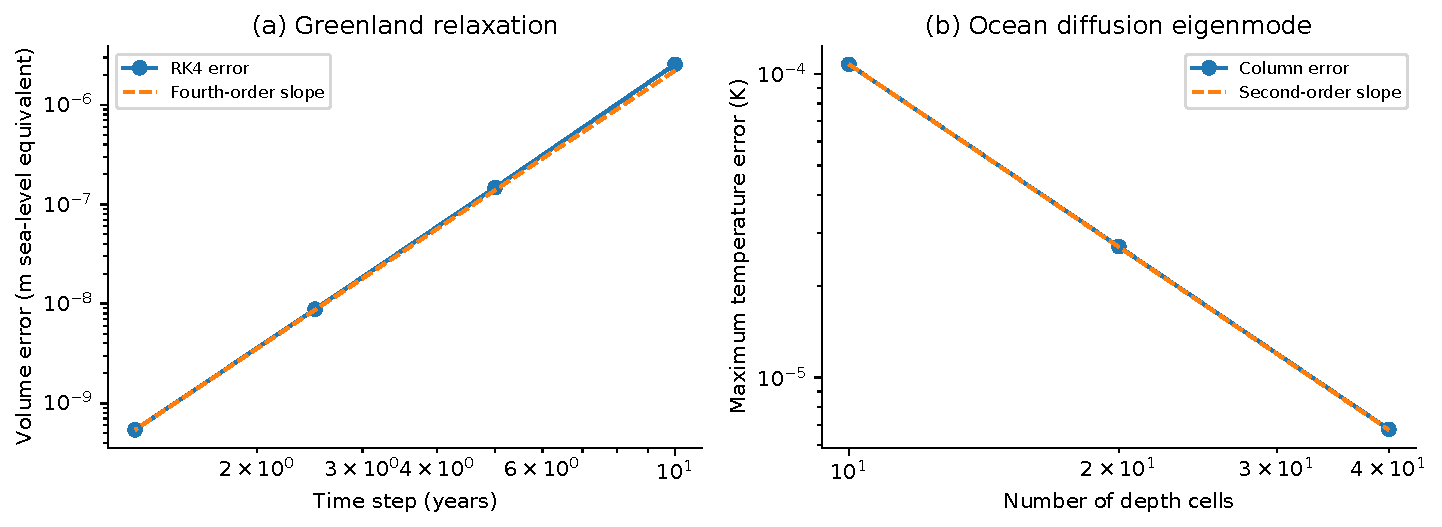
\includegraphics[width=\textwidth]{diagnostic_convergence.pdf}
\caption{Independent convergence tests. (a) Greenland volume error at 100 years
against the exact exponential relaxation; the dashed line has fourth-order
slope. (b) Maximum ocean temperature error at 0.2\,s for 10, 20 and 40 cells;
the dashed line has second-order slope. Time step is 0.2 divided by the square
of the cell count, in seconds.}\label{fig:convergence}
\end{figure}

\subsection{Flood-loss integration and decision sensitivity}

Figure\ref{fig:flood} uses a manufactured 5\,km$^2$ segment distributed uniformly
over 0--5\,m elevation. Capital density is one million USD\,km$^{-2}$, population
density 100\,km$^{-2}$, mortality fraction 0.01, value of life 100,000 USD and
resilience 0.2. These values are verification fixtures, not recommended valuations.
The GEV parameters are location 1\,m, scale 0.3\,m and shape 0.1. The outer integral
extends from $-2$ to 20\,m. SciPy uses its opposite-sign shape convention and
independent adaptive integration for both elevation and surge. This verifies
the Julia closed-form depth integral and composite-Simpson expectation.

\begin{figure}[htbp]\centering
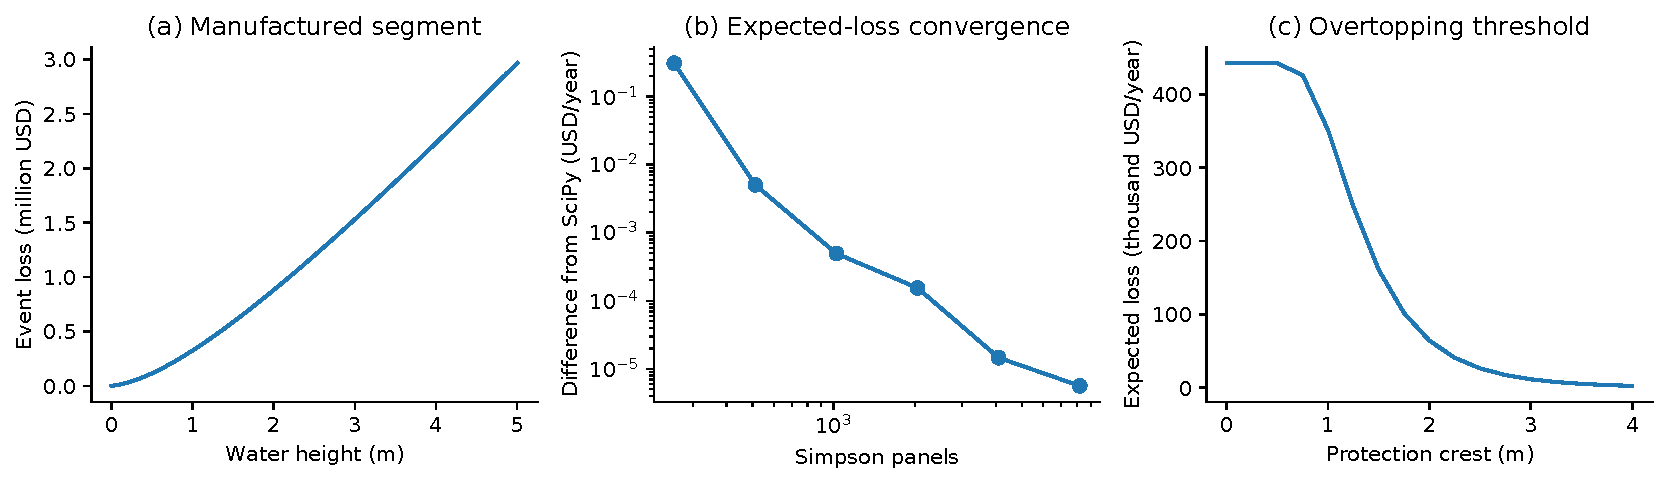
\includegraphics[width=\textwidth]{diagnostic_flood.pdf}
\caption{Manufactured coastal damage verification. (a) Event damage increases
with water height. (b) Expected annual loss approaches an independent nested
SciPy integral as the number of Simpson panels increases. (c) Expected
overtopping loss decreases with protection crest. Panel(c) omits construction
cost and therefore is not an optimal seawall-height calculation.}\label{fig:flood}
\end{figure}

Table\ref{tab:decision} quantifies two accounting ambiguities with manufactured
costs. A two-period menu has candidate costs $(1, 9)$ and $(6, 2)$ at years 2010
and 2060. Keeping one candidate differs from allowing a switch. This menu has
no inherited infrastructure state; it is a test of the decision rule only.
Likewise, ten annual unit payments during 2010--2019 differ from paying ten
units at either end. A coarse timestep must retain the annual-flow interpretation
if it is to reproduce the same present value.

\begin{table}[htbp]\centering
\begin{tabular}{lr}\toprule
Manufactured accounting choice & Present value\\\midrule
fixed strategy pv & 2.266414 \\
revisable strategy pv & 1.281425 \\
ten annual unit payments pv & 8.435332 \\
ten units paid at start pv & 10.000000 \\
ten units paid at end pv & 7.025867 \\

\bottomrule\end{tabular}
\caption{Sensitivity to strategy persistence and payment timing at 4\% annual
discounting. Units are arbitrary currency; these are not coastal estimates.}
\label{tab:decision}
\end{table}

\subsection{Antarctic transform and its asserted floor}

For $a>0$ and $x<0$, the added term in Equation\ref{eq:anto} is negative.
The literal transformation therefore falls below $T_f$, despite its description
as bounded below by freezing \cite{brick}. For the test values $a=1,b=0$, the
minimum is approximately $-2.07846$\,$^\circ$C. In dimensionless form,
$z=x/a$, the extremum satisfies $1+e^{-z}+ze^{-z}=0$, giving
$z\simeq-1.27846$ and a minimum increment $-0.27846a$.
Figure\ref{fig:anto} shows this algebraic behavior. No freezing clamp was added.
Whether the calibrated historical trajectory visits this regime remains unknown.

\begin{figure}[htbp]\centering
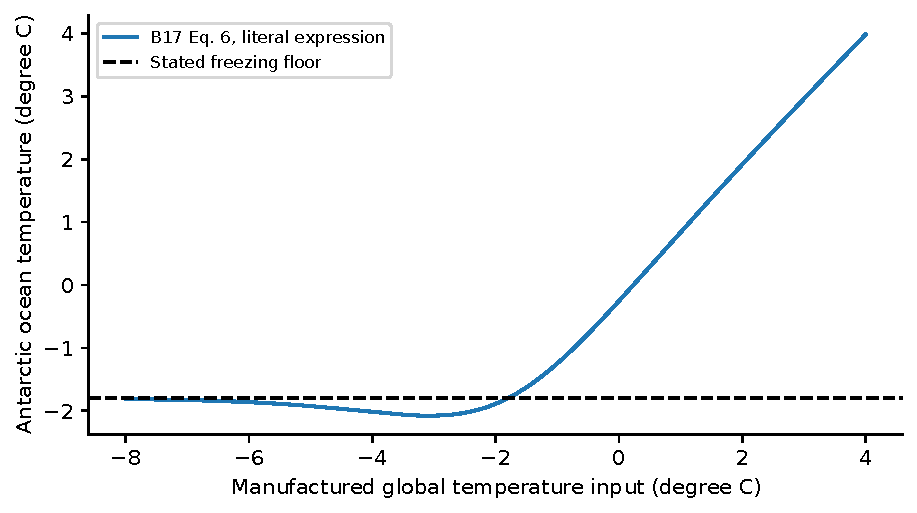
\includegraphics[width=.73\textwidth]{diagnostic_anto.pdf}
\caption{Literal BRICK Antarctic ocean-temperature transformation with
manufactured coefficients $a=1,b=0$ and stated freezing temperature
$-1.8$\,$^\circ$C. The curve falls below the dashed floor for negative $x$.
This is a specification diagnostic, not an Antarctic projection.}\label{fig:anto}
\end{figure}

\section{Quantitative comparison boundary}

The target reports median costs of 1.2, 1.5, 2.1 and 2.6 trillion 2010 USD across the
four warming bins, with fifth percentiles 1.0, 1.2, 1.6 and 2.2 trillion USD
\cite{wong2025}. The prose supplies 95th percentiles 1.3 and 2.3 trillion USD
for the first two bins; unreported numerical endpoints were not digitized or
invented. No independent global costs exist here, so neither relative errors nor
agreement intervals can be calculated for those targets.

An arithmetic audit of the printed Table 1 is possible. Its four counts sum to
5,000. Among 250 simulations above 2.7 trillion USD, the text gives 125 in the
highest bin and 109 in the third, with none in the lowest. The remaining 16
belong to the second bin. Dividing these counts by bin size yields the rounded
probabilities in the paper (Table\ref{tab:audit}). This verifies internal
consistency of printed summaries; it does not reproduce the modeled probability
distribution or establish an independently calculated tail threshold.

\begin{table}[htbp]\centering
\begin{tabular}{rrrrr}\toprule
Bin & Printed count & Tail count & Calculated\% & Printed\%\\\midrule
1 & 202 & 0 & 0.0000 & 0 \\
2 & 2264 & 16 & 0.7067 & 1 \\
3 & 2145 & 109 & 5.0816 & 5 \\
4 & 389 & 125 & 32.1337 & 32 \\

\bottomrule\end{tabular}
\caption{Arithmetic audit using published counts only. The second-bin tail
count 16 is derived by subtraction. These data never enter the model kernels.}
\label{tab:audit}
\end{table}

\section{Complete figure-by-figure record}

Table\ref{tab:status} covers all main and supplementary figures and the main
table. Unlettered joint and marginal views are listed separately. Every entry's
dependencies, source provenance, assumptions, commands, comparison status and
failure explanation are also recorded in \texttt{docs/FIGURE\_STATUS.csv}.
For unavailable outputs, the generation command is explicitly unavailable;
there is no plotting command that can turn missing model predictions into an
independent reproduction. Supplementary Figure 10 is one histogram containing
all-member and Antarctic-trigger-conditioned distributions of proactive migrants.

\small
\begin{longtable}{p{.22\textwidth}p{.48\textwidth}p{.22\textwidth}}
\caption{Target reproduction status. ``Not reproduced'' means no independently
generated target numerical result.}\label{tab:status}\\
\toprule Figure/view & Quantity & Status\\\midrule\endfirsthead
\toprule Figure/view & Quantity & Status\\\midrule\endhead
1: global interval plot & Conditional median and 5th-95th cost quantiles & Not reproduced \\
2: joint scatter & Sea level 2100 versus discounted costs & Not reproduced \\
2: top marginal & Sea level distribution by warming bin & Not reproduced \\
2: right marginal & Cost distribution by warming bin & Not reproduced \\
3: regional bars & Regional cost/GDP minus global cost/GDP & Not reproduced \\
4: workflow & Model components and exchanges & Conceptual schematic \\
S1: interval plot & 5000 versus 4000 subsample comparison & Not reproduced \\
S2: interval plot & 202 per bin versus full sample & Not reproduced \\
S3: trajectory plot & GMST median and 90\% intervals plus AR6 boxes & Not reproduced \\
S4: trajectory plot & GMSL median and 66\% intervals plus AR6 boxes & Not reproduced \\
S5: map & Median local sea level 2100 & Not reproduced \\
S6: interval plot & GTSR versus DINAS cost intervals & Not reproduced \\
S7: joint scatter & Sea level versus costs above 2.7 trillion & Not reproduced \\
S7: top marginal & Upper-tail sea level distribution & Not reproduced \\
S7: right marginal & Upper-tail cost distribution & Not reproduced \\
S8: regional bars & SSP2 regional cost/GDP deviations & Not reproduced \\
S9: regression plot & Regional SSP income contrast versus cost sensitivity & Not reproduced \\
S10: histograms & Migration conditional on AIS trigger & Not reproduced \\
Table1: table & Warming-bin counts and tail probabilities & Not reproduced \\

\bottomrule
\end{longtable}
\normalsize

Main Figure 1 requires full conditional cost distributions. Figure 2 requires
joint sea-level/cost realizations, and Figure 3 additionally requires regional
economic aggregation. Supplementary Figures 1 and 2 require controlled subsampling
of a legitimate ensemble, not merely a sample-size calculation. Figures 3 and 4
require calibrated time series plus AR6 comparisons. Figure 5 requires spatial
fingerprints and site matching. Figure 6 requires matched GTSR and DINAS extreme
levels. Figure 7 requires the original type of upper-tail joint distribution.
Figures 8 and 9 require paired SSP2/SSP4 economics. Figure 10 requires retained
segment migration histories and Antarctic-trigger states. The implemented
summary and aggregation routines do not supply these missing physical inputs.

\section{Continued recovery, implementation and observational experiments}
\label{sec:continuation}

The earlier assessment identified missing mechanisms too broadly. Reading the
complete Tanaka thesis and the 2022 scholarly preprint recovered the DOECLIM
constants, the coastal decision menu and the socioeconomic priors. Independent
providers supplied forcing, temperature, carbon emissions, ocean heat and
coastal-hazard inputs \cite{inputs}. The active audit in
\texttt{docs/BLOCKER\_AUDIT.md} distinguishes recovered specifications,
derived corrections, explicit alternatives and remaining data gaps.

\subsection{Coupled energy balance and numerical heat transport}

The land--troposphere and ocean--troposphere boxes exchange heat and lose energy
through separate radiative feedbacks \cite{tanaka,urban}. For land fraction
$f=0.29$, their temperatures $T_L,T_S$ satisfy
\begin{align}
C_L\dot T_L&=Q-\lambda_LT_L-\frac{k}{f}(T_L-bT_S),\\
C_S\dot T_S&=Q-\lambda_ST_S+\frac{k}{1-f}(T_L-bT_S)-F_O.
\end{align}
Here $b=1.3$, $C_L=0.52$ and $C_S=7.8$\,W\,yr\,m$^{-2}$\,K$^{-1}$.
The global surface-air observable is $fT_L+(1-f)bT_S$. The equilibrium land/SST
ratio is 1.43 and $k=1.59-0.31\lambda_L$. Together with an equilibrium warming
of ECS under 3.7\,W\,m$^{-2}$, these relations determine both feedbacks and the
exchange coefficient. The explicit formulas are recorded in
\texttt{docs/RECOVERED\_SPECIFICATIONS.md}.

An 80-cell, 4000\,m interior ocean exchanges heat continuously with the mixed
layer and has an insulated bottom. Finite-volume fluxes cancel under a global
heat-capacity weighted sum; this is tested independently of equilibrium fitting.
Crank--Nicolson integration uses four steps per year. Refining the vertical grid
from 80 to 160 cells changes the year-70 warming under 1\% annual CO$_2$ growth
by 0.000787\,K; the next doubling changes it by 0.000197\,K. This approximately
fourfold error reduction agrees with second-order spatial convergence.

The 60\,m effective mixed-layer capacity contains about 2.5\,m of
atmospheric-equivalent capacity. Comparisons with NOAA integrate only 57.5\,m
of water and the appropriate fractional interior cells down to the stated
observational depth. Whole-column heat is not compared to a 700\,m record.
HadCRUT4 blends land air temperature with SST, whereas the legacy DOECLIM
observable includes enhanced marine-air warming. Treating that blended record
as the global-air observable follows the simplified legacy calibration and is
an additional representation approximation, not an exact observation operator.

\subsection{A closed, explicitly alternative carbon cycle}

The recovered terrestrial stocks are 100, 500, 120 and 1500\,Gt\,C in leaves,
wood, detritus and soil \cite{siegenthaler}. Baseline NPP of 60\,Gt\,C\,yr$^{-1}$
allocates 35 to leaves and 25 to wood. Leaf turnover sends 35 to detritus;
wood sends 20 to detritus and 5 to soil. Detritus respires 45 and transfers 10
to soil; soil respires 15. Linear turnover rates are these fluxes divided by
their source stocks. Fertilization modifies NPP and the documented $Q_{10}$
factor modifies the two respiration fluxes \cite{ricciuto}. All internal
transfers cancel in the global carbon balance.

Ocean carbon uses an instantaneously equilibrated atmosphere--mixed-layer
reservoir and three deeper reservoirs. Constant alkalinity, total boron and
carbonate equilibrium determine atmospheric CO$_2$ and mixed-layer carbon from
their combined inventory \cite{hooss1999}. The nonlinear scalar root is solved
by bisection in log hydrogen concentration. At 280\,ppm the reconstructed DIC
is 0.002080909\,mol\,L$^{-1}$, consistent with the printed H99 value to its
reported precision. The mixed-layer depth and deep exchange parameters are
from the later Tanaka description. Mixing these documented versions, and
holding carbonate chemistry temperature fixed, defines an alternative closure;
it does not establish exact recovery of the target SNEASY version.

Second-order splitting couples carbon RK4 steps to climate CN steps. Twenty-six
checks establish baseline equilibrium, chemical partition, stock positivity,
second-order coupled convergence and total-carbon conservation. Across 18
historical sensitivities, the largest carbon-budget residual is below
$10^{-11}$\,Gt\,C. Conservation alone does not validate the response: the
uncalibrated default predicts 461.38\,ppm in 2022, compared with NOAA's
417.08\,ppm. The GCB historical table has no pre-1850 land-use emissions; the
input retains blanks, while separate calculations prescribe zero or the 1850
rate before 1850. These are alternatives, not recovered observations.

\begin{figure}[htbp]
\centering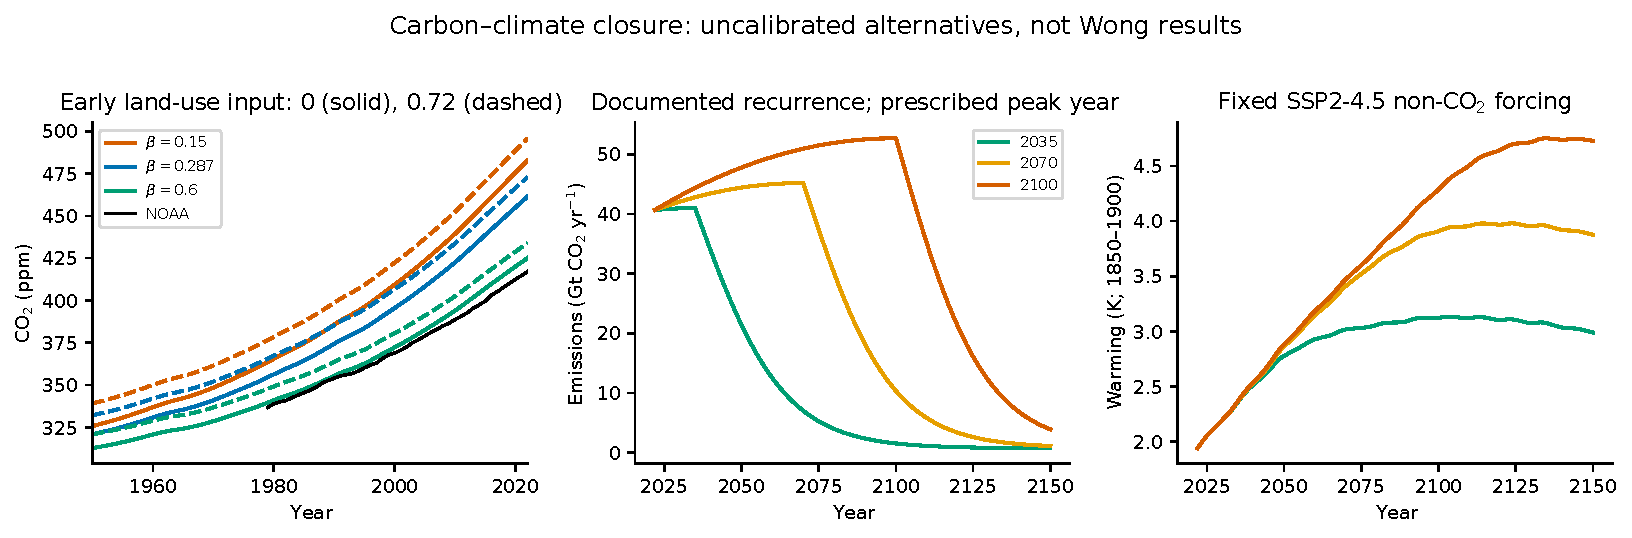
\includegraphics[width=\textwidth]{carbon_alternative.pdf}
\caption{Uncalibrated carbon--climate experiments, not target reproductions.
Left: historical CO$_2$ sensitivities to fertilization and the explicitly
assumed early land-use input, with independent NOAA observations. Centre:
documented emissions recurrence initialized from GCB2023, with three prescribed
peak years. Right: coupled warming under fixed SSP2-4.5 non-CO$_2$ forcing.
The historical mismatch limits interpretation of these future curves.}
\end{figure}

\subsection{Temperature-only calibration and failed holdout checks}

The first observational experiment estimates ECS, heat diffusivity, aerosol
multiplier, temperature offset, AR1 innovation scale and AR1 correlation.
HadCRUT4.6.0.0 years 1850--2005 form the training data; years 2006--2021 are
held out. Known observational standard deviations are approximated by the total
95\% interval widths divided by $2(1.96)$. This approximation omits the record's
full temporally correlated measurement covariance. A scalar Kalman filter
integrates the latent AR1 residual exactly under these assumptions; tests match
the dense Gaussian covariance likelihood to $10^{-12}$.

Uniform bounds follow the B17 climate table, except that ECS is restricted to
0.7--10\,K: the recovered exchange relation becomes negative below about
0.68\,K. CEDA effective forcing supplies historical and future inputs, with
both aerosol components multiplied by the same parameter. This differs from
the older indirect-aerosol convention and from Darnell's uncertain emissions
and nearest-SSP forcing construction. Neither the posterior nor the six
scenario experiments is claimed as the Wong ensemble.

An initial short run failed convergence checks. The retained calculation uses
four dispersed chains, each with 6000 warmup and 30,000 production steps;
every fifth state is retained. Proposal adaptation stops before production.
Log ECS and log diffusivity proposals include their Jacobian, preserving the
physical-coordinate prior. Independently implemented rank/folded split
$\widehat R$ and bulk/tail ESS follow Vehtari et al.\ \cite{vehtari}.
The largest $\widehat R$ is 1.00427 and the smallest ESS is 1894, satisfying
the prespecified limits of 1.01 and 400.

Conditional forecasts propagate the final training-period residual state and
include both AR1 innovation and observational uncertainty. Despite sampler
convergence, holdout temperature RMSE is 0.209\,K, with mean bias
$+0.189$\,K. Only 10 of 16 held-out annual temperatures lie inside the nominal
90\% predictive intervals. After fitting only an additive heat datum offset
over 1955--2005, the 700\,m heat parameter-median RMSE in 2006--2021 is
$16.46\times10^{22}$\,J. These failures motivate a separate temperature--heat
calibration; they are not removed from the record.

One thousand complete joint parameter rows generate six SSP trajectories;
250- and 500-row subsets test sampling variation. The physical temperature
intervals exclude future residual noise. SSP2-4.5 mean warming over
2081--2100 is 2.924\,K, with a parameter 90\% interval of 1.976--4.188\,K.
The corresponding printed AR6 assessment is 2.7 [2.1, 3.5]\,K. This comparison
uses the same averaging/reference periods but compares different inference
systems; it is not a numerical reproduction of Supplementary Figure S3.

\begin{figure}[htbp]
\centering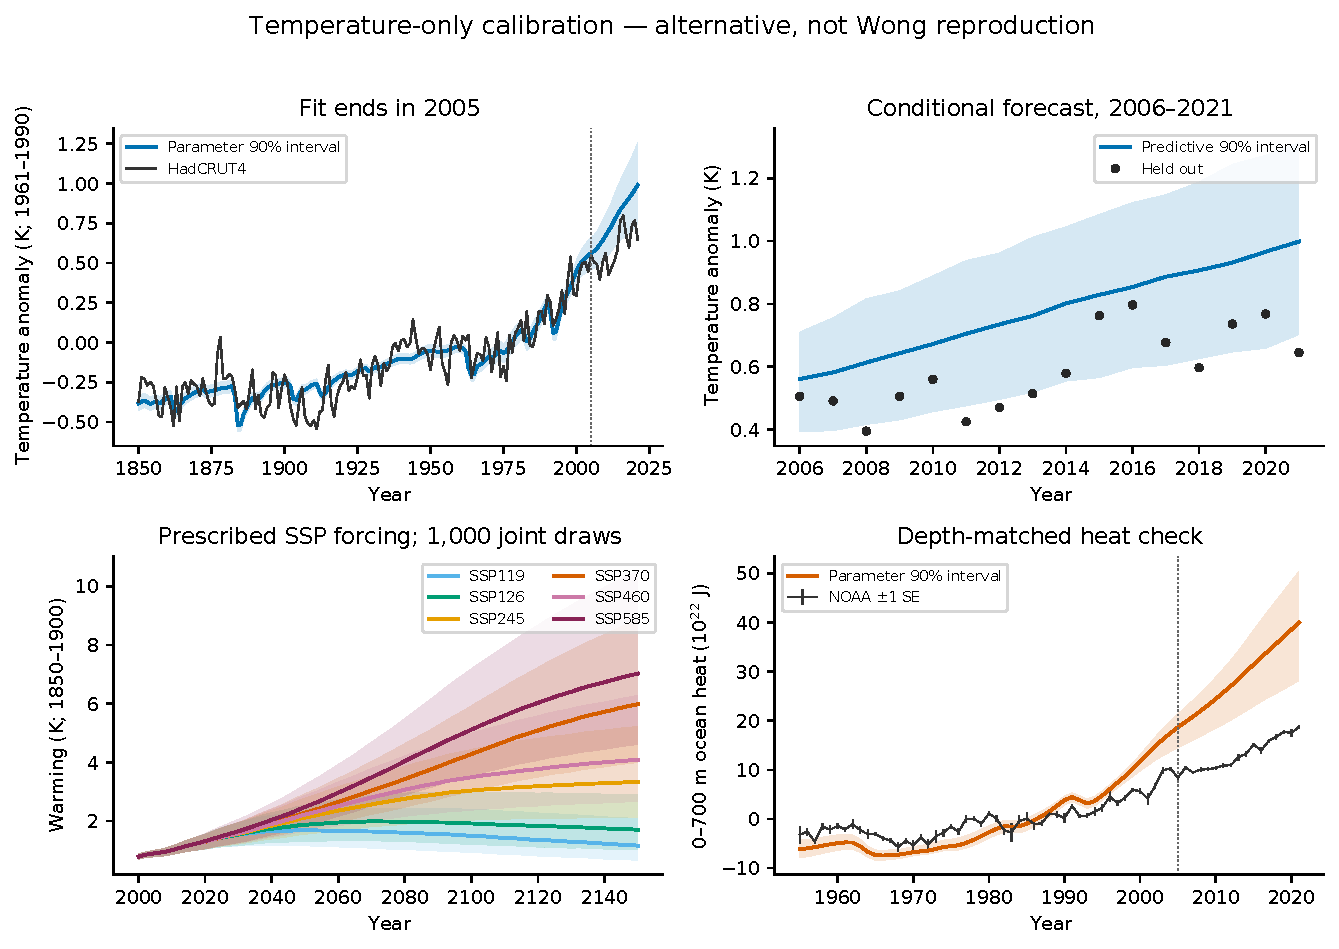
\includegraphics[width=\textwidth]{climate_alternative.pdf}
\caption{Temperature-only calibration and independent observational checks.
The upper-right forecast includes residual and measurement uncertainty. The
lower-left scenario bands contain parameter uncertainty only. Ocean heat is
compared at the actual observational depth, with a training-period datum offset.
The temperature and heat holdout discrepancies prevent treating this converged
alternative posterior as validation of the target model.}
\end{figure}

\subsection{Joint temperature--heat calibration}

The next experiment adds independent NOAA 0--700\,m heat observations over
1955--2005, with a datum offset and separate AR1 residual parameters. The
first joint run failed convergence ($\widehat R=1.0218$ and a heat-correlation
ESS of about 285). Its diagnostics remain in the repository. A revised
sampler uses logarithmic innovation scales, logit correlations and a recent
warmup covariance window; Jacobians preserve the same physical priors.
Four chains of 8000 warmup and 50,000 production iterations retain 20,000
states. All acceptance checks pass: the maximum $\widehat R$ is 1.00582 and
the minimum bulk/tail ESS is 589.

An exact modal solver reduces computation while retaining all finite-volume
degrees of freedom. A diagonal similarity transforms the climate operator
into a symmetric tridiagonal matrix. Each mode is integrated analytically
under linearly interpolated annual forcing. Eighteen checks agree with an
independent augmented matrix exponential and establish second-order
Crank--Nicolson convergence. Four substeps per year differ from the exact
solution by at most 0.00133\,K in three historical comparisons; the exact
solver is used consistently for the new joint fit and projections.

The joint fit reduces held-out temperature RMSE to 0.0870\,K and bias to
$+0.0402$\,K. Heat predictive RMSE is $0.879\times10^{22}$\,J. All 16 held-out
years lie in both nominal 90\% predictive intervals. These short, correlated
holdouts provide limited validation; coverage is not a proof of correct
uncertainty. ECS has a median of 1.485\,K and a parameter 90\% interval of
1.093--1.958\,K. Future warming is substantially below the AR6 assessment:
SSP2-4.5 warming over 2081--2100 is 1.973 [1.518,2.483]\,K, compared with
2.7 [2.1,3.5]\,K; SSP5-8.5 is 3.319 [2.569,4.160]\,K, compared with
4.4 [3.3,5.7]\,K. This discrepancy remains unresolved. Improved historical
prediction does not justify replacing the target's joint climate--carbon--ice
calibration with this alternative.

\begin{figure}[htbp]
\centering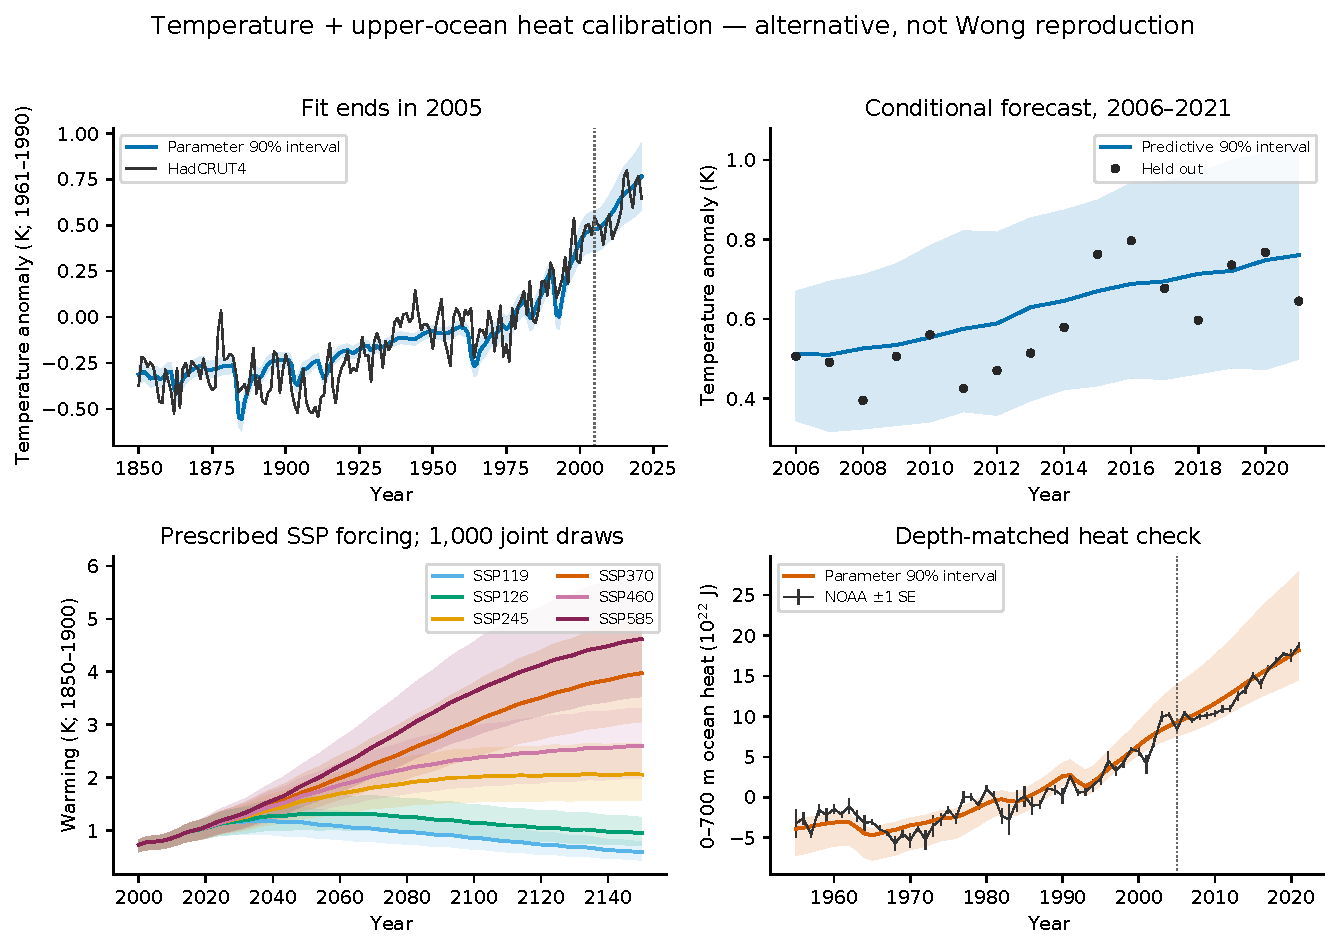
\includegraphics[width=\textwidth]{climate_joint_alternative.pdf}
\caption{Alternative joint temperature and upper-ocean-heat calibration.
Observations after 2005 are withheld. Future bands propagate parameter
uncertainty under prescribed SSP forcing. The improved holdout performance
and the low late-century warming relative to AR6 are both retained.}
\end{figure}

\subsection{Antarctic events and observational thermal expansion}

DAIS geometry, accumulation and marine discharge are now implemented. The
discharge water depth follows sea level minus bed elevation, correcting the
printed sign from geometry; coefficient units follow dimensional consistency.
The equilibrium volume of $2.478479\times10^{16}$\,m$^3$ differs from Shaffer's
rounded $2.478\times10^{16}$\,m$^3$ by 0.0193\%. This is a reproduced
methodological benchmark, not a reproduced Wong figure.

The printed runoff gate activates at $h_0+cT_A=0$. Over marine bed this can
produce a discontinuous accumulation rate. Splitting time steps at that event
and evaluating endpoint stages on the appropriate side removes the earlier
irregular refinement. In the 6\,K, century-long warming ramp, the event occurs
at year 41.92982456. Two-year and one-year steps differ in year-200 radius by
$1.57\times10^{-7}$\,m; finer steps reach floating-point limits. The dashed
curves in Figure\ref{fig:recovered} instead activate runoff when the runoff
line exceeds local edge height, and remain explicit alternative physics.
These tests express sea level by mass conservation using ice/water densities
and ocean area, whereas B17 scales its initial Antarctic volume to 57\,m.
The two observable conventions are not silently interchanged.

\begin{figure}[htbp]
\centering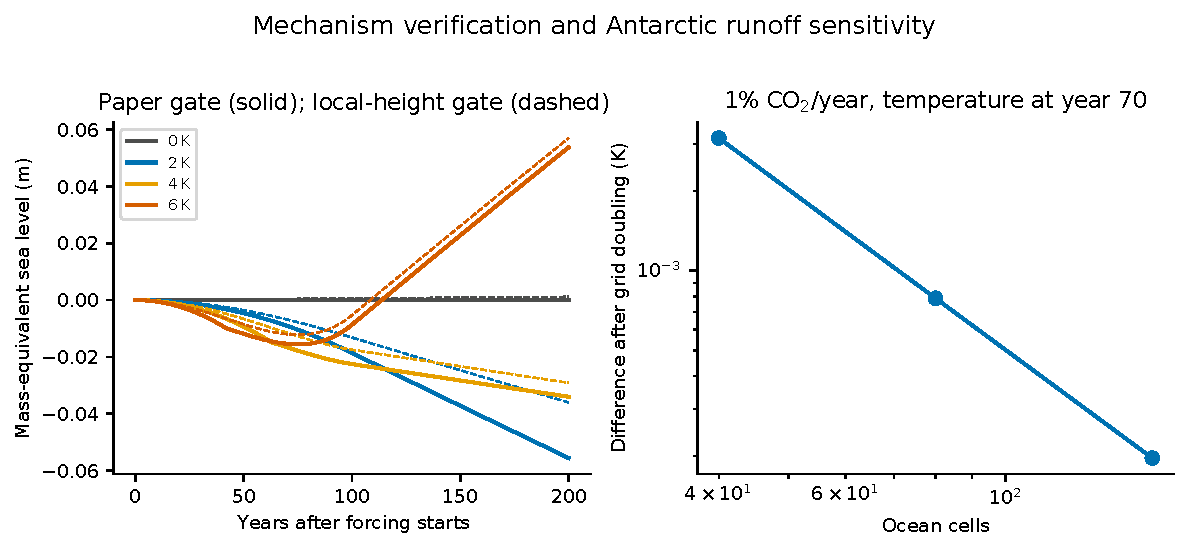
\includegraphics[width=.98\textwidth]{recovered_mechanisms.pdf}
\caption{Independent mechanism tests. Left: prescribed Antarctic warming,
with fixed ocean temperature and sea level, isolates the runoff convention.
Right: climate grid refinement under 1\% annual CO$_2$ growth. Neither panel
is a global calibrated projection.}\label{fig:recovered}
\end{figure}

An independent coefficient check uses NOAA heat and thermosteric sea level
from the same depth range. OLS over 1955--2005 at 0--700\,m gives
$1.392\times10^{-25}$\,m\,J$^{-1}$; fitting 2005--2015 at 0--2000\,m gives
$1.107\times10^{-25}$\,m\,J$^{-1}$. Held-out thermosteric RMSEs through 2021
are 0.414 and 0.757\,mm, respectively. First-difference slopes provide a check
against merely fitting a common trend. Because heat and sea level share
hydrographic observations, these are descriptive constraints rather than
independent-error coefficient posteriors. They are not substituted silently
for the unavailable V19 prior or a full-depth expansion coefficient.

\begin{figure}[htbp]
\centering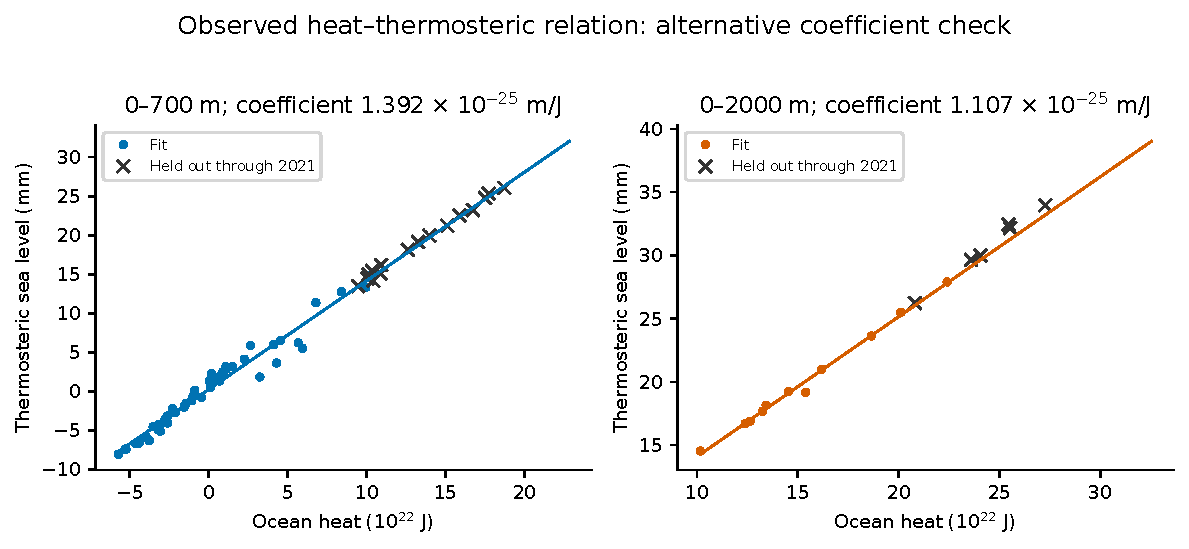
\includegraphics[width=.98\textwidth]{thermal_observations.pdf}
\caption{Independent NOAA heat and thermosteric observations with fitted
depth-specific linear relations. Later years through 2021 were withheld.
This coefficient check is an explicit alternative to the target calibration.}
\end{figure}

\subsection{Coastal cash flows and input quality}

The annual coastal experiment retains the documented ten-choice menu and
first-period decision rule. Sixty checks establish nonnegative cash-flow
components, first-period policy selection, no repeated relocation at fixed
sea level and telescoping incremental dike construction costs. Upgrades at
2010, 2051 and 2101, annual payment timing and a paired no-SLR counterfactual
are explicit alternatives to the target's decadal accounting and initial-step
subtraction. Forty-eight synthetic scenarios compare income/exposure, sea-level
rise, retreat land accounting and linear versus quadratic maintenance.
All exposure values are labeled fixtures; no global cost estimate is inferred.
Doubling flood quadrature from 512 to 1024 panels changes the verification-case
NPV by about 0.00024\,USD and leaves its policy unchanged.

\begin{figure}[htbp]
\centering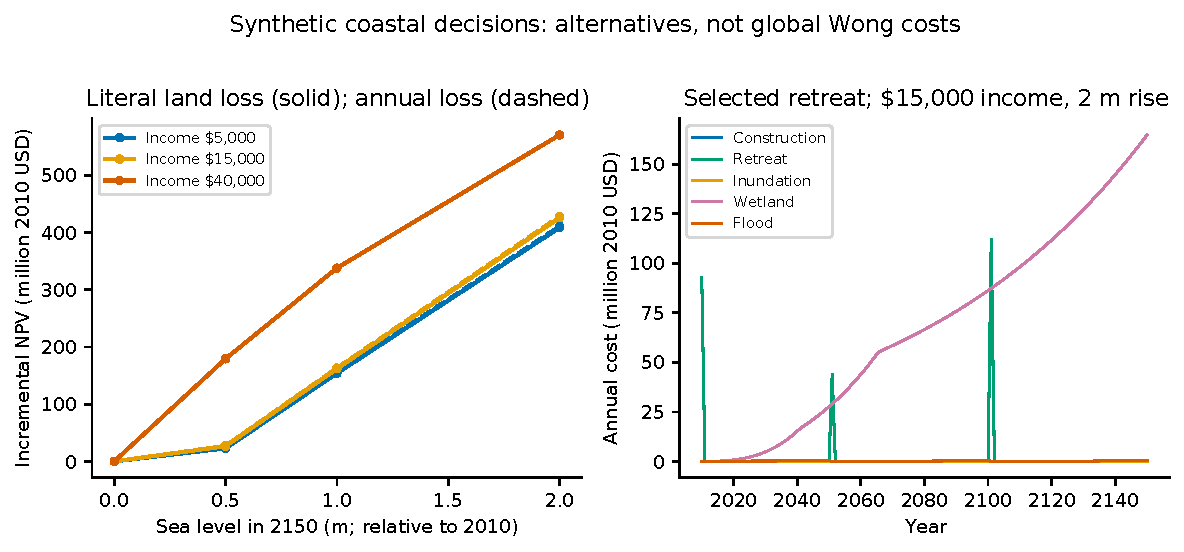
\includegraphics[width=.98\textwidth]{coastal_alternative.pdf}
\caption{Synthetic coastal alternatives. Left: paired-counterfactual incremental
costs under two explicit land-accounting rules. Income and exposure both vary
across the three fixtures, so this is not an isolated income effect.
Right: annual components for one selected retreat policy, including discrete
upgrades. These outputs do not estimate a named coast or a global cost.}
\end{figure}

The independent GTSR shapefile has 12,148 coastal feature rows but only 7868
distinct station labels. The initial interpretation of these labels as unique
DIVA identifiers was corrected by this audit. A second public release provides
16,611 station-wise Gumbel fits. Geographic mapping leaves 133 nearest matches
with invalid parameters; these remain missing, not filled from distant stations.
The two input products also disagree in their 100-year levels. These findings
prevent a silent merge or assumption of exact input equivalence. The full
target elevation-area, exposure and DINAS tide records still require recovery.
The next section uses a separately sourced geographic input product for an
explicit alternative, with different segmentation and monetary conventions.

Every alternative here has its own input, script, output and figure record.
No alternative curve is entered into the target inventory as a recovered
published numerical result. Ongoing calibration and data-recovery tasks remain
active rather than being reclassified as irreducible merely because the first
implementation lacked them.


\section{Unresolved inputs and implications}

The joint parameter distribution is a central missing scientific object.
The cited methodology combines paleo Antarctic constraints, modern climate
and component-sea-level observations, uncertain emissions, and autoregressive
residuals. Complete target likelihood definitions, data vintages, measurement
errors, initial states, and residual treatment were not recovered. Reusing
published posterior samples is prohibited here. Independent calibration is now
being performed with versioned exogenous observations and explicitly alternative
likelihood choices. Independent draws from older marginal quantiles would
discard physically relevant dependence.

The historical DIVA exposure bundle is another independent obstacle. The CIAM
supplement reports that its v1.5.5 database was no longer supported and that
v1.8 was not public at that time \cite{diaz}. The EEA provider directory currently
reports unavailable software \cite{diva}. This does not prove that every DIVA
dataset is inaccessible; it establishes that a complete permissible target
bundle was not recovered in this investigation. No modern coastline segmentation
was substituted for the 12,148 target segments.

Independent GTSR data and six SSP forcing inputs have been acquired
\cite{gtsr,ssp}. The GTSR release supplies coastal features and a later release
supplies Gumbel parameters, but invalid records, repeated station labels and
return-level discrepancies require explicit treatment. The 2022 academic
supplement was recovered in the scholarly preprint, resolving the six
socioeconomic marginal priors and several decision conventions. Country
economics, original elevation-area/exposure data, component fingerprints and
the precise target data vintages remain unresolved.

The active stages are therefore to extend the independent calibration, reconcile
the remaining carbon/ice variants, and recover permissible segment and economic
inputs. Small coupled experiments precede any target-sized ensemble. No result in this report
supports a quantitative conclusion about the target's regional cost inequality.

\section{Assessment of the research-agent process}

The agent recovered much of the mathematical interface from distributed
scholarly sources, distinguished versions of a mutable preprint, and implemented
several independently checkable numerical components. The analytical tests
separate solver accuracy from calibration and data availability. Cross-language
flood integration supplies an additional check against transcription or
implementation errors in the elevation primitive and GEV convention.

Two interpretation errors were avoided through source comparison. First, the
older BRICK temperature-based expansion emulator is not the heat-based component
described in the target lineage. Second, a later revision behind the same DOI
cannot automatically be treated as the manuscript available before publication.
Direct calculation then identified two tensions between printed equations and
their prose descriptions. These checks do not reveal the original implementation.

The principal limitation is evidence recovery, not numerical throughput.
An agent can write functioning code while failing to identify the scientific
experiment if it supplies convenient values for missing inputs. This project
does not count such code as a successful reproduction. The initial assessment
stopped too early: further scholarly reading recovered major mechanisms and
independent inputs. Observation-based calibration, carbon mass closure and DAIS
integration are now demonstrated, while a global adaptation ensemble remains
unreproduced. The failed holdout checks show why solver verification and posterior
convergence cannot substitute for validation of the predicted observable.

The research log records source access failures, incidental search exposure,
interpretation decisions, and verification outcomes. No subagents were used.
The work followed Brad Lipovsky's supplied research instructions and academic
style guide. This assessment concerns the recorded execution; it is not a
general benchmark of all AI research systems.

\section{Reproducibility and current scope}

Run \texttt{bash scripts/run\_all.sh} from the project root to execute the
offline verification, generate numerical diagnostics and figures, and compile
this report. Julia uses standard libraries only. Python 3.6.8, NumPy 1.19.5,
SciPy 1.5.4 and Matplotlib 3.3.4 were available locally; pdfLaTeX comes from
TeXLive 2018. The driver verifies executable availability and imports, requires
no installation, and limits numerical libraries to one thread. Calculations
run at scheduling priority 19 on a heavily loaded shared server. All artifacts,
temporary files and tool caches are directed into the designated project.
Source acquisition is a separate optional, hash-checked command. The scientific
build does not require network access or downloaded authors' outputs.

The independent calculations verify response and cost mechanisms, quantify
written-specification discrepancies, and test alternative observation-conditioned
climate scenarios. An original conceptual
Figure 4 is complete. Main Figures 1--3, supplementary Figures 1--10 and modeled
Table 1 remain unreproduced. A printed-table arithmetic agreement is not promoted
to numerical-model agreement. The missing calibration and coastal inputs must
be resolved before an assessment of the target scientific conclusions can be
claimed. These remaining tasks do not invalidate the completed mechanism tests
or authorize treating this progress report as project completion.

\begin{thebibliography}{99}
\bibitem{wong2025} Wong, T. E., Dake, S., Feke, K., Darnell, C., and Srikrishnan, V.
(2025). Coastal adaptation and damage costs at different global warming
thresholds. \emph{npj Natural Hazards}, 2, 35.
\href{https://doi.org/10.1038/s44304-025-00089-0}{doi:10.1038/s44304-025-00089-0}.
Includes seven-page supplementary information.
\bibitem{darnell} Darnell, C., and coauthors (2024 manuscript revision).
The interplay of future emissions and geophysical uncertainties for future sea level rise.
\href{https://doi.org/10.31219/osf.io/j47ts}{doi:10.31219/osf.io/j47ts}.
Original scholarly file kt9av, revision 9, deposited 11 December 2024;
\href{https://osf.io/download/kt9av/?revision=9}{versioned manuscript}.
The citation's exact manuscript revision is unresolved.
\bibitem{urban} Urban, N. M., and Keller, K. (2010).
Probabilistic hindcasts and projections of the coupled climate, carbon cycle
and Atlantic meridional overturning circulation system: a Bayesian fusion
of century-scale observations with a simple model. \emph{Tellus A}, 62,737--750.
\href{https://doi.org/10.1111/j.1600-0870.2010.00471.x}{doi:10.1111/j.1600-0870.2010.00471.x}.
\bibitem{ricciuto} Ricciuto, D. M., Davis, K. J., and Keller, K. (2008).
A Bayesian calibration of a simple carbon cycle model: the role of observations
in estimating and reducing uncertainty. \emph{Global Biogeochemical Cycles}, 22.
\href{https://doi.org/10.1029/2006GB002908}{doi:10.1029/2006GB002908}.
\bibitem{brick} Wong, T. E., and coauthors (2017).
BRICK v0.2, a simple, accessible, and transparent model framework for climate
and regional sea-level projections. \emph{Geoscientific Model Development}, 10, 2741--2760.
\href{https://doi.org/10.5194/gmd-10-2741-2017}{doi:10.5194/gmd-10-2741-2017}.
\bibitem{joss} Wong, T. E., and coauthors (2022). MimiBRICK.jl: a Julia package
for the BRICK model for sea-level change in the Mimi integrated modeling framework.
\emph{Journal of Open Source Software}.
\href{https://doi.org/10.21105/joss.04556}{doi:10.21105/joss.04556}.
Written article consulted; software was not consulted.
\bibitem{shaffer} Shaffer, G. (2014). Formulation, calibration and validation
of the DAIS model (version 1), a simple Antarctic ice sheet model sensitive to
variations of sea level and ocean subsurface temperature.
\emph{Geoscientific Model Development}, 7, 1803--1818.
\href{https://doi.org/10.5194/gmd-7-1803-2014}{doi:10.5194/gmd-7-1803-2014}.
\bibitem{diaz} Diaz, D. B. (2016). Estimating global damages from sea level rise
with the Coastal Impact and Adaptation Model (CIAM). \emph{Climatic Change}.
\href{https://doi.org/10.1007/s10584-016-1675-4}{doi:10.1007/s10584-016-1675-4}.
Mathematical specification in supplementary information, pp.9--17.
\bibitem{vega} Vega-Westhoff, B., Sriver, R. L., Hartin, C. A., Wong, T. E., and
Keller, K. (2019). Impacts of observational constraints related to sea level
on estimates of climate sensitivity. \emph{Earth's Future}, 7,677--690.
\href{https://doi.org/10.1029/2018EF001082}{doi:10.1029/2018EF001082}.
\bibitem{wong2022} Wong, T. E., and coauthors (2022). Sea level and
socioeconomic uncertainty drives high-end coastal adaptation costs. \emph{Earth's Future}.
\href{https://doi.org/10.1029/2022EF003061}{doi:10.1029/2022EF003061}.
\bibitem{diva} European Environment Agency, Climate-ADAPT. Dynamic Interactive
Vulnerability Assessment model (DIVA), provider directory, accessed 12 October 2026.
\href{https://climate-adapt.eea.europa.eu/en/metadata/tools/dynamic-interactive-vulnerability-assessment-model-diva}{Provider record}.
\bibitem{gtsr} Muis, S., Verlaan, M., Winsemius, H. C., Aerts, J. C. J. H.,
and Ward, P. J. (2016). A global reanalysis of storm surges and extreme sea
levels. \emph{Nature Communications}, 7, 11969.
\href{https://doi.org/10.1038/ncomms11969}{doi:10.1038/ncomms11969}.
Dataset provenance checked at Vrije Universiteit Amsterdam and 4TU.
\bibitem{ssp} IIASA. Shared Socioeconomic Pathways Scenario Database.
\href{https://iiasa.ac.at/models-tools-data/ssp}{Provider documentation},
accessed 12 October 2026. Multiple GDP interpretations and data vintages require
explicit selection before a target reconstruction.
\bibitem{tanaka} Tanaka, K. (2008). Inverse estimation for the simple Earth
system model ACC2. Doctoral thesis. Chapter 2 supplies physical equations;
software appendices were not consulted.
\href{https://pure.mpg.de/rest/items/item_2389991_2/component/file_2389990/content}{Scholarly thesis}.
\bibitem{siegenthaler} Siegenthaler, U., and Oeschger, H. (1987).
Biospheric CO$_2$ emissions during the past 200 years reconstructed by
deconvolution of ice core data. \emph{Tellus B}, 39, 140--154.
\href{https://b.tellusjournals.se/articles/1693/files/submission/proof/1693-1-15260-1-10-20221121.pdf}{Published methods and reservoir diagram}.
\bibitem{hooss1999} Hooss, G., and coauthors (1999). A nonlinear impulse
response model of the coupled carbon cycle--climate system (NICCS).
MPI scientific report, carbon chemistry section.
\href{https://climatehomes.unibe.ch/~joos/papers/hooss99mpi.pdf}{Scholarly report}.
\bibitem{vehtari} Vehtari, A., Gelman, A., Simpson, D., Carpenter, B., and
Buerkner, P.-C. (2021). Rank-normalization, folding, and localization:
an improved $\widehat R$ for assessing convergence of MCMC.
\emph{Bayesian Analysis}. \href{https://doi.org/10.1214/20-BA1221}{doi:10.1214/20-BA1221}.
\bibitem{inputs} Independent input providers. Met Office HadCRUT4.6.0.0
(Morice et al., 2012); CEDA radiative forcing (Smith, 2023); CMIP6 concentrations
(Meinshausen et al., 2020); NOAA GML CO$_2$ (Lan et al.); NOAA NCEI ocean heat
and thermosteric sea level (Levitus et al., 2012); Global Carbon Budget 2023
(Friedlingstein et al., 2023). Exact citations, units, licenses, subset
definitions and versioned hashes are in \texttt{inputs/README.md} and
\texttt{docs/EXTERNAL\_INPUTS.csv}.
\end{thebibliography}
\end{document}
